\chapter{Os cinco sentidos}\label{ch:g1:the-five-senses}

Feche os \omterm{def:g1:the-five-senses:sense}{olhos} e o mundo não some: você continua ouvindo a sala,
sentindo o cheiro do almoço, sentindo a cadeira embaixo de você. O
corpo tem cinco portas para o mundo --- os sentidos --- e cada porta
é um órgão do corpo, trabalhando para você o dia inteiro.

\section{Cinco sentidos, cinco órgãos}

\begin{definition}[Sentido e órgão do sentido]\label{def:g1:the-five-senses:sense}
Um \emph{sentido}\index{sentido} é um jeito que o corpo tem de
descobrir o mundo. Cada sentido funciona por meio de um \emph{órgão
do sentido}\index{órgão do sentido}, uma parte do corpo feita para
esse trabalho:
\begin{enumerate}
  \item a \emph{visão}\index{visão} --- os \emph{olhos}\index{olho}
        veem a luz, as cores e as formas;
  \item a \emph{audição}\index{audição} --- os
        \emph{ouvidos}\index{ouvido} escutam os sons;
  \item o \emph{olfato}\index{olfato} --- o \emph{nariz}\index{nariz}
        sente os cheiros;
  \item o \emph{paladar}\index{paladar} --- a
        \emph{língua}\index{língua} sente o gosto da comida;
  \item o \emph{tato}\index{tato} --- a \emph{pele}\index{pele},
        no corpo inteiro, sente o áspero e o liso, o quente e o frio.
\end{enumerate}
\end{definition}

\begin{example}[O café da manhã, sentido por sentido]\label{ex:g1:the-five-senses:breakfast}
Uma tigela de chocolate quente usa os cinco: os \omterm{def:g1:the-five-senses:sense}{olhos} veem o
vaporzinho, o nariz sente o cheiro do cacau, a \omterm{def:g1:the-five-senses:sense}{pele} das mãos sente a
tigela morna, os \omterm{def:g1:the-five-senses:sense}{ouvidos} escutam a colher tilintar e a língua --- a
melhor parte --- sente o gosto.
\end{example}

\begin{omfigure}
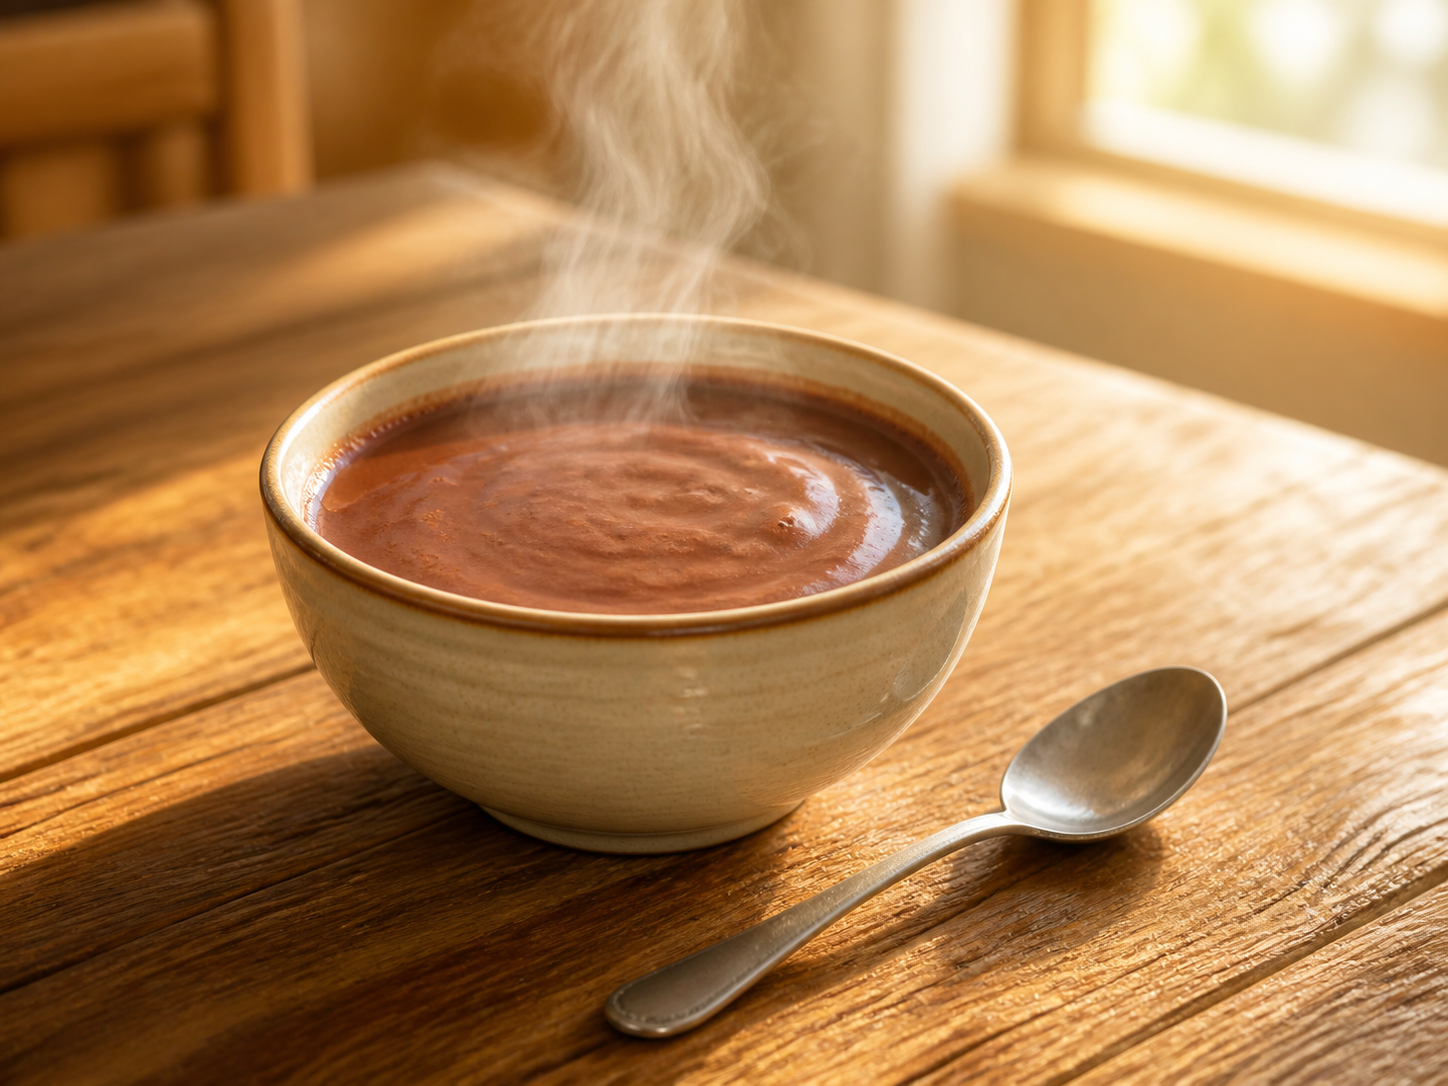
\includegraphics[width=0.58\linewidth]{images/book1/ai/g1-senses-chocolate.png}

{\small Uma tigela de chocolate quente, cinco sentidos trabalhando
antes do primeiro gole.}
\end{omfigure}

\begin{remark}[O tato está em toda parte]\label{rem:g1:the-five-senses:skin}
Quatro \omterm{def:g1:the-five-senses:sense}{órgãos dos sentidos} moram na cabeça, mas o órgão do tato é a
\omterm{def:g1:the-five-senses:sense}{pele}, e a \omterm{def:g1:the-five-senses:sense}{pele} cobre você da cabeça aos pés. É por isso que você
sente uma brisa no pescoço, uma pedrinha dentro do sapato e uma
joaninha pousando no seu \omterm{def:g1:my-body:parts}{braço} --- tudo isso sem olhar.
\end{remark}

\section{Os sentidos avisam o cérebro}

\begin{proposition}[Mensagens para o cérebro]\label{prop:g1:the-five-senses:brain}
Um \omterm{def:g1:the-five-senses:sense}{órgão do sentido} não entende o que sente --- ele \emph{manda uma
mensagem}. Todas as mensagens viajam por dentro do corpo até o
\emph{cérebro}\index{cérebro}, na cabeça, que junta tudo: ``essa é a
voz da vovó'', ``esse cheiro é de torrada''. Sem o cérebro, os \omterm{def:g1:the-five-senses:sense}{olhos}
e os \omterm{def:g1:the-five-senses:sense}{ouvidos} não avisariam ninguém.
\end{proposition}
\admitted

\begin{omfigure}
\begin{tikzpicture}[scale=0.9]
  % brain box
  \draw[thick, omDef, fill=omDef!8, rounded corners=6pt]
    (4.6,0.2) rectangle (8.2,2.0);
  \node[font=\small\bfseries, omDef] at (6.4,1.55) {o cérebro};
  \node[font=\small, align=center, text width=3.2cm] at (6.4,0.85)
    {junta as\\ mensagens};
  % organs
  \node[font=\small, left] (eye) at (2.2,2.6) {o olho vê};
  \node[font=\small, left] (ear) at (2.2,1.7) {o ouvido escuta};
  \node[font=\small, left] (nose) at (2.2,0.8) {o nariz cheira};
  \node[font=\small, left] (skin) at (2.2,-0.1) {a pele sente};
  % arrows
  \draw[->, thick, omMeth] (2.35,2.55) -- (4.55,1.75);
  \draw[->, thick, omMeth] (2.35,1.68) -- (4.55,1.35);
  \draw[->, thick, omMeth] (2.35,0.82) -- (4.55,0.95);
  \draw[->, thick, omMeth] (2.35,-0.02) -- (4.55,0.55);
  \node[font=\small, omMeth] at (3.4,3.0) {mensagens};
\end{tikzpicture}

{\small Cada \omterm{def:g1:the-five-senses:sense}{órgão do sentido} manda a sua mensagem para o cérebro,
que dá sentido a todas elas. (A língua também avisa --- só que o
desenho ficaria cheio demais.)}
\end{omfigure}

\begin{example}[Adivinhar no escuro]\label{ex:g1:the-five-senses:dark}
Um amigo põe um objeto conhecido nas suas mãos com os \omterm{def:g1:the-five-senses:sense}{olhos}
fechados: uma chave, uma esponja, uma colher. Você diz o nome quase
na hora. A \omterm{def:g1:the-five-senses:sense}{pele} mandou a mensagem --- frio, duro, cheio de pontas
--- e o cérebro respondeu: ``uma chave''. Os sentidos recolhem; o
cérebro entende.
\end{example}

\begin{remark}[Ajudando uns aos outros]\label{rem:g1:the-five-senses:together}
Os sentidos trabalham em equipe. A comida parece sem graça quando um
resfriado entope o nariz, porque o olfato estava fazendo metade do
trabalho do sabor. E, quando um sentido não consegue fazer o
trabalho dele, os outros aprendem a fazer mais: quem não enxerga lê
com a ponta dos dedos, usando o tato, e atravessa a rua com os
\omterm{def:g1:the-five-senses:sense}{ouvidos}.
\end{remark}

\section{Cuidar dos órgãos dos sentidos}

\begin{proposition}[Portas frágeis]\label{prop:g1:the-five-senses:fragile}
Os \omterm{def:g1:the-five-senses:sense}{órgãos dos sentidos} são preciosos e fáceis de machucar. Som alto
demais machuca os \omterm{def:g1:the-five-senses:sense}{ouvidos}; olhar para o Sol machuca os \omterm{def:g1:the-five-senses:sense}{olhos}; uma
colherada quente demais queima a língua. Um \omterm{def:g1:the-five-senses:sense}{órgão do sentido}
machucado pode ficar machucado para sempre --- por isso a gente
protege esses órgãos.
\end{proposition}
\admitted

\begin{method}[Proteger os meus sentidos]\label{met:g1:the-five-senses:protect}
\begin{enumerate}
  \item Nunca olhe direto para o Sol, nem por um instante;
  \item mantenha os sons suaves: nada de gritar no \omterm{def:g1:the-five-senses:sense}{ouvido} dos
        outros, e fone de \omterm{def:g1:the-five-senses:sense}{ouvido} em volume baixo;
  \item nunca enfie nada no \omterm{def:g1:the-five-senses:sense}{ouvido} nem no nariz;
  \item assopre a comida quente antes de provar;
  \item leia e desenhe com boa luz.
\end{enumerate}
\end{method}

\begin{example}[O show do vizinho]\label{ex:g1:the-five-senses:loud}
Depois de uma música muito alta, os \omterm{def:g1:the-five-senses:sense}{ouvidos} às vezes ficam apitando
um tempo. Esse apito é o \omterm{def:g1:the-five-senses:sense}{ouvido} dizendo ``foi demais!''. Quem
trabalha com máquinas barulhentas usa protetor de \omterm{def:g1:the-five-senses:sense}{ouvido} exatamente
por isso --- os \omterm{def:g1:the-five-senses:sense}{ouvidos} têm que durar a vida inteira.
\end{example}

\section{Exercícios}

\begin{exercise}[$\star$]\label{exo:g1:the-five-senses:1}
Diga os cinco sentidos e, para cada um, o \omterm{def:g1:the-five-senses:sense}{órgão do sentido} dele.
\end{exercise}

\begin{exercise}[$\star$]\label{exo:g1:the-five-senses:2}
Qual \omterm{def:g1:the-five-senses:sense}{órgão do sentido} avisa: (a) a cor de um balão? (b) a maciez de
um cobertor? (c) o cheiro de chuva? (d) o som de um sino?
\end{exercise}

\begin{exercise}[$\star$]\label{exo:g1:the-five-senses:3}
Qual \omterm{def:g1:the-five-senses:sense}{órgão do sentido} não fica na cabeça? Até onde ele vai?
\end{exercise}

\begin{exercise}[$\star$]\label{exo:g1:the-five-senses:4}
No \cref{ex:g1:the-five-senses:dark}, os \omterm{def:g1:the-five-senses:sense}{olhos} estavam fechados.
Qual órgão mandou a mensagem, e qual parte do corpo entendeu?
\end{exercise}

\begin{exercise}[$\star$]\label{exo:g1:the-five-senses:5}
Com um resfriado e o nariz entupido, a comida parece perder o sabor.
Quais dois sentidos costumam fazer dupla na hora de comer?
\end{exercise}

\begin{exercise}[$\star$]\label{exo:g1:the-five-senses:6}
Dê três regras do \cref{met:g1:the-five-senses:protect} e diga qual
\omterm{def:g1:the-five-senses:sense}{órgão do sentido} cada uma protege.
\end{exercise}

\begin{exercise}[$\star$]\label{exo:g1:the-five-senses:7}
Por que quem trabalha com máquinas barulhentas usa protetor de
\omterm{def:g1:the-five-senses:sense}{ouvido}? Use a \cref{prop:g1:the-five-senses:fragile}.
\end{exercise}

\begin{exercise}[$\star$]\label{exo:g1:the-five-senses:8}
Faça a experiência: de \omterm{def:g1:the-five-senses:sense}{olhos} fechados, peça a alguém para segurar
três alimentos debaixo do seu nariz --- talvez banana, queijo,
laranja. Quantos o seu nariz acertou, sem a ajuda dos \omterm{def:g1:the-five-senses:sense}{olhos}?
\end{exercise}

\begin{exercise}[$\star\star$]\label{exo:g1:the-five-senses:9}
Um amigo afirma: ``O \omterm{def:g1:the-five-senses:sense}{olho} entende o que vê.'' Corrija a frase usando
a \cref{prop:g1:the-five-senses:brain}: o que o \omterm{def:g1:the-five-senses:sense}{olho} faz de verdade,
e quem é que entende?
\end{exercise}

\begin{exercise}[$\star\star$]\label{exo:g1:the-five-senses:10}
Como uma pessoa que não enxerga consegue ``ler'' um livro e
atravessar a rua com segurança? Diga quais sentidos assumem quais
trabalhos.
\end{exercise}
